\chapter{Задача коммивояжера}

Решить задачу коммивояжера с 10 городами.

\begin{center}
    \begin{tabular}{|a | c | c | c | c | c | c | c | c | c | c|} 
         \hline
         \rowcolor{LightGray}
            & 1 & 2 & 3 & 4 & 5 & 6 & 7 & 8 & 9 & 10\\
         \hline
            1 & \cellcolor{Beige}$\infty$ & 13 & 16 & 44 & 27 & 71 & 38 & 62 & 83 & 33\\
         \hline
            2 & 31 & \cellcolor{Beige}$\infty$ & 43 & 96 & 18 & 83 & 25 & 79 & 12 & 22\\
         \hline
            3 & 18 & 12 & \cellcolor{Beige}$\infty$ & 89 & 33 & 26 & 41 & 37 & 77 & 94\\
         \hline
            4 & 63 & 46 & 71 & \cellcolor{Beige}$\infty$ & 92 & 47 & 59 & 84 & 32 & 15\\
        \hline
            5 & 23 & 57 & 79 & 34 & \cellcolor{Beige}$\infty$ & 42 & 83 & 79 & 95 & 42\\
         \hline
            6 & 57 & 11 & 28 & 65 & 34 & \cellcolor{Beige}$\infty$ & 40 & 74 & 39 & 53\\
         \hline
            7 & 96 & 38 & 50 & 29 & 82 & 49 & \cellcolor{Beige}$\infty$ & 51 & 22 & 19\\
         \hline
            8 & 66 & 48 & 72 & 58 & 93 & 41 & 54 & \cellcolor{Beige}$\infty$ & 70 & 53\\
        \hline
            9 & 73 & 13 & 56 & 89 & 31 & 23 & 45 & 30 & \cellcolor{Beige}$\infty$ & 92\\
         \hline
            10 & 60 & 47 & 77 & 55 & 99 & 44 & 55 & 38 & 16 & \cellcolor{Beige}$\infty$\\
        \hline
    \end{tabular}
\end{center}

\begin{center}
    {\bf
    Решение:}
\end{center}

\begin{center}
    \begin{tabular}{|a | c | c | c | c | c | c | c | c | c | c | g|} 
         \hline
         \rowcolor{LightGray}
            & 1 & 2 & 3 & 4 & 5 & 6 & 7 & 8 & 9 & 10 & min\\
         \hline
            1 & \cellcolor{Beige}$\infty$ & 13 & 16 & 44 & 27 & 71 & 38 & 62 & 83 & 33 & 13\\
         \hline
            2 & 31 & \cellcolor{Beige}$\infty$ & 43 & 96 & 18 & 83 & 25 & 79 & 12 & 22 & 12\\
         \hline
            3 & 18 & 12 & \cellcolor{Beige}$\infty$ & 89 & 33 & 26 & 41 & 37 & 77 & 94 & 12\\
         \hline
            4 & 63 & 46 & 71 & \cellcolor{Beige}$\infty$ & 92 & 47 & 59 & 84 & 32 & 15 & 15\\
        \hline
            5 & 23 & 57 & 79 & 34 & \cellcolor{Beige}$\infty$ & 42 & 83 & 79 & 95 & 42 & 23\\
         \hline
            6 & 57 & 11 & 28 & 65 & 34 & \cellcolor{Beige}$\infty$ & 40 & 74 & 39 & 53 & 11\\
         \hline
            7 & 96 & 38 & 50 & 29 & 82 & 49 & \cellcolor{Beige}$\infty$ & 51 & 22 & 19 & 19\\
         \hline
            8 & 66 & 48 & 72 & 58 & 93 & 41 & 54 & \cellcolor{Beige}$\infty$ & 70 & 53 & 41\\
        \hline
            9 & 73 & 13 & 56 & 89 & 31 & 23 & 45 & 30 & \cellcolor{Beige}$\infty$ & 92 & 13\\
         \hline
            10 & 60 & 47 & 77 & 55 & 99 & 44 & 55 & 38 & 16 & \cellcolor{Beige}$\infty$ & 16\\
        \hline
    \end{tabular}
\end{center}

\begin{center}
    \begin{tabular}{|a | c | c | c | c | c | c | c | c | c | c|} 
         \hline
         \rowcolor{LightGray}
            & 1 & 2 & 3 & 4 & 5 & 6 & 7 & 8 & 9 & 10\\
         \hline
            1 & \cellcolor{Beige}$\infty$ & 0 & 3 & 31 & 14 & 58 & 25 & 49 & 70 & 20\\
         \hline
            2 & 19 & \cellcolor{Beige}$\infty$ & 31 & 84 & 6 & 71 & 13 & 67 & 0 & 10\\
         \hline
            3 & 6 & 0 & \cellcolor{Beige}$\infty$ & 77 & 21 & 14 & 29 & 25 & 65 & 82\\
         \hline
            4 & 48 & 31 & 56 & \cellcolor{Beige}$\infty$ & 77 & 32 & 44 & 69 & 17 & 0\\
        \hline
            5 & 0 & 34 & 56 & 11 & \cellcolor{Beige}$\infty$ & 19 & 60 & 56 & 72 & 19\\
         \hline
            6 & 46 & 0 & 17 & 54 & 23 & \cellcolor{Beige}$\infty$ & 29 & 63 & 28 & 42\\
         \hline
            7 & 77 & 19 & 31 & 10 & 63 & 30 & \cellcolor{Beige}$\infty$ & 32 & 3 & 0\\
         \hline
            8 & 25 & 7 & 31 & 17 & 52 & 0 & 13 & \cellcolor{Beige}$\infty$ & 29 & 12\\
        \hline
            9 & 60 & 0 & 43 & 76 & 18 & 10 & 32 & 17 & \cellcolor{Beige}$\infty$ & 79\\
         \hline
            10 & 44 & 31 & 61 & 39 & 83 & 28 & 39 & 22 & 0 & \cellcolor{Beige}$\infty$\\
        \hline
        \rowcolor{LightBlue}
            min & 0 & 0 & 3 & 10 & 6 & 0 & 13 & 17 & 0 & 0\\
         \hline
    \end{tabular}
\end{center}

Нижняя граница издержек - сумма приводящих констант:\\
$h = (13 + 12 + 12 + 15 + 23 + 11 + 19 + 41 + 13 + 16) + (3 + 10 + 6 + 13 + 17) = 224$\\
$G_0$ - множество всех маршрутов\\
$w(G_0) = h = 224$

\begin{center}
    \begin{tabular}{|a | c | c | c | c | c | c | c | c | c | c | g|} 
         \hline
         \rowcolor{LightGray}
            & 1 & 2 & 3 & 4 & 5 & 6 & 7 & 8 & 9 & 10 & \\
         \hline
            1 & \cellcolor{Beige}$\infty$ & 0 & 0 & 21 & 8 & 58 & 12 & 32 & 70 & 20 & 0\\
         \hline
            2 & 19 & \cellcolor{Beige}$\infty$ & 28 & 74 & 0 & 71 & 0 & 50 & 0 & 10 & 0\\
         \hline
            3 & 6 & 0 & \cellcolor{Beige}$\infty$ & 67 & 15 & 14 & 16 & 8 & 65 & 82 & 6\\
         \hline
            4 & 48 & 31 & 53 & \cellcolor{Beige}$\infty$ & 71 & 32 & 31 & 52 & 17 & 0 & 17\\
        \hline
            5 & 0 & 34 & 53 & 1 & \cellcolor{Beige}$\infty$ & 19 & 47 & 39 & 72 & 19 & 1\\
         \hline
            6 & 46 & 0 & 14 & 44 & 17 & \cellcolor{Beige}$\infty$ & 16 & 46 & 28 & 42 & 14\\
         \hline
            7 & 77 & 19 & 28 & 0 & 57 & 30 & \cellcolor{Beige}$\infty$ & 15 & 3 & 0 & 0\\
         \hline
            8 & 25 & 7 & 28 & 7 & 46 & 0 & 0 & \cellcolor{Beige}$\infty$ & 29 & 12 & 0\\
        \hline
            9 & 60 & 0 & 40 & 66 & 12 & 10 & 19 & 0 & \cellcolor{Beige}$\infty$ & 79 & 0\\
         \hline
            10 & 44 & 31 & 58 & 29 & 77 & 28 & 26 & 5 & 0 & \cellcolor{Beige}$\infty$ & 5\\
        \hline
        \rowcolor{LightBlue}
             & 6 & 0 & 14 & 1 & 8 & 10 & 0 & 5 & 0 & 0 &\\
         \hline
    \end{tabular}
\end{center}

Претенденты на ветвление:\\
$S_{12}, S_{13}, S_{25}, S_{27}, S_{29}, S_{32}, S_{4,10}, S_{51}, S_{62}, S_{74}, S_{7,10}, S_{86}, S_{87}, S_{92}, S_{98}, S_{10,9} = 0$\\
$Q_{12} = 0 + 0 = 0$\\
$Q_{13} = 14 + 0 = 0$\\
$Q_{25} = 8 + 0 = 8$\\
$Q_{27} = 0 + 0 = 0$\\
$Q_{29} = 0 + 0 = 0$\\
$Q_{32} = 0 + 6 = 6$\\
$Q_{4,10} = 0 + 17 = 17$\\
$Q_{51} = 0 + 1 = 1$\\
$Q_{62} = 0 + 14 = 14$\\
$Q_{74} = 1 + 0 = 1$\\
$Q_{7,10} = 0 + 0 = 0$\\
$Q_{86} = 10 + 0 = 10$\\
$Q_{87} = 0 + 0 = 0$\\
$Q_{92} = 0 + 0 = 0$\\
$Q_{98} = 5 + 0 = 5$\\
$Q_{10,9} = 0 + 5 = 5$\\

$Q_{max} = Q_{4,10} = 17 \implies$ выбираем для ветвления пару (4, 10)\\
$w(\overline{\{4, 10\}}) = 224 + 17 = 241$

\begin{center}
    \begin{tabular}{|a | c | c | c | c | c | c | c | c | c |} 
         \hline
         \rowcolor{LightGray}
            & 1 & 2 & 3 & 4 & 5 & 6 & 7 & 8 & 9 \\
         \hline
            1 & \cellcolor{Beige}$\infty$ & 0 & 0 & 21 & 8 & 58 & 12 & 32 & 70 \\
         \hline
            2 & 19 & \cellcolor{Beige}$\infty$ & 28 & 74 & 0 & 71 & 0 & 50 & 0 \\
         \hline
            3 & 6 & 0 & \cellcolor{Beige}$\infty$ & 67 & 15 & 14 & 16 & 8 & 65 \\
         \hline
            5 & 0 & 34 & 53 & 1 & \cellcolor{Beige}$\infty$ & 19 & 47 & 39 & 72 \\
         \hline
            6 & 46 & 0 & 14 & 44 & 17 & \cellcolor{Beige}$\infty$ & 16 & 46 & 28 \\
         \hline
            7 & 77 & 19 & 28 & 0 & 57 & 30 & \cellcolor{Beige}$\infty$ & 15 & 3 \\
         \hline
            8 & 25 & 7 & 28 & 7 & 46 & 0 & 0 & \cellcolor{Beige}$\infty$ & 29 \\
        \hline
            9 & 60 & 0 & 40 & 66 & 12 & 10 & 19 & 0 & \cellcolor{Beige}$\infty$ \\
         \hline
            10 & 44 & 31 & 58 & \cellcolor{Beige}$\infty$ & 77 & 28 & 26 & 5 & 0\\
        \hline
    \end{tabular}
\end{center}

\begin{center}
    \begin{tabular}{|a | c | c | c | c | c | c | c | c | c | g|} 
         \hline
         \rowcolor{LightGray}
            & 1 & 2 & 3 & 4 & 5 & 6 & 7 & 8 & 9 & min \\
         \hline
            1 & \cellcolor{Beige}$\infty$ & 0 & 0 & 21 & 8 & 58 & 12 & 32 & 70 & 0\\
         \hline
            2 & 19 & \cellcolor{Beige}$\infty$ & 28 & 74 & 0 & 71 & 0 & 50 & 0 & 0\\
         \hline
            3 & 6 & 0 & \cellcolor{Beige}$\infty$ & 67 & 15 & 14 & 16 & 8 & 65 & 0 \\
         \hline
            5 & 0 & 34 & 53 & 1 & \cellcolor{Beige}$\infty$ & 19 & 47 & 39 & 72 & 0 \\
         \hline
            6 & 46 & 0 & 14 & 44 & 17 & \cellcolor{Beige}$\infty$ & 16 & 46 & 28 & 0\\
         \hline
            7 & 77 & 19 & 28 & 0 & 57 & 30 & \cellcolor{Beige}$\infty$ & 15 & 3 & 0 \\
         \hline
            8 & 25 & 7 & 28 & 7 & 46 & 0 & 0 & \cellcolor{Beige}$\infty$ & 29 & 0 \\
        \hline
            9 & 60 & 0 & 40 & 66 & 12 & 10 & 19 & 0 & \cellcolor{Beige}$\infty$ & 0 \\
         \hline
            10 & 44 & 31 & 58 & \cellcolor{Beige}$\infty$ & 77 & 28 & 26 & 5 & 0 & 0\\
        \hline
    \end{tabular}
\end{center}

\begin{center}
    \begin{tabular}{|a | c | c | c | c | c | c | c | c | c |} 
         \hline
         \rowcolor{LightGray}
            & 1 & 2 & 3 & 4 & 5 & 6 & 7 & 8 & 9 \\
         \hline
            1 & \cellcolor{Beige}$\infty$ & 0 & 0 & 21 & 8 & 58 & 12 & 32 & 70 \\
         \hline
            2 & 19 & \cellcolor{Beige}$\infty$ & 28 & 74 & 0 & 71 & 0 & 50 & 0 \\
         \hline
            3 & 6 & 0 & \cellcolor{Beige}$\infty$ & 67 & 15 & 14 & 16 & 8 & 65 \\
         \hline
            5 & 0 & 34 & 53 & 1 & \cellcolor{Beige}$\infty$ & 19 & 47 & 39 & 72 \\
         \hline
            6 & 46 & 0 & 14 & 44 & 17 & \cellcolor{Beige}$\infty$ & 16 & 46 & 28 \\
         \hline
            7 & 77 & 19 & 28 & 0 & 57 & 30 & \cellcolor{Beige}$\infty$ & 15 & 3 \\
         \hline
            8 & 25 & 7 & 28 & 7 & 46 & 0 & 0 & \cellcolor{Beige}$\infty$ & 29 \\
        \hline
            9 & 60 & 0 & 40 & 66 & 12 & 10 & 19 & 0 & \cellcolor{Beige}$\infty$ \\
         \hline
            10 & 44 & 31 & 58 & \cellcolor{Beige}$\infty$ & 77 & 28 & 26 & 5 & 0\\
        \hline
        \rowcolor{LightBlue}
             min & 0 & 0 & 0 & 0 & 0 & 0 & 0 & 0 & 0\\
         \hline
    \end{tabular}
\end{center}

Сумма приводящих констант: $h = 0 + 0 = 0$\\
$w(\{4, 10\}) = 224 + 0 = 224 < 241 \implies$ включаем (4, 10) в маршрут

\begin{center}
    \begin{tabular}{|a | c | c | c | c | c | c | c | c | c | g|} 
         \hline
         \rowcolor{LightGray}
            & 1 & 2 & 3 & 4 & 5 & 6 & 7 & 8 & 9 &  \\
         \hline
            1 & \cellcolor{Beige}$\infty$ & 0 & 0 & 21 & 8 & 58 & 12 & 32 & 70 & 0\\
         \hline
            2 & 19 & \cellcolor{Beige}$\infty$ & 28 & 74 & 0 & 71 & 0 & 50 & 0 & 0\\
         \hline
            3 & 6 & 0 & \cellcolor{Beige}$\infty$ & 67 & 15 & 14 & 16 & 8 & 65 & 6 \\
         \hline
            5 & 0 & 34 & 53 & 1 & \cellcolor{Beige}$\infty$ & 19 & 47 & 39 & 72 & 1 \\
         \hline
            6 & 46 & 0 & 14 & 44 & 17 & \cellcolor{Beige}$\infty$ & 16 & 46 & 28 & 14\\
         \hline
            7 & 77 & 19 & 28 & 0 & 57 & 30 & \cellcolor{Beige}$\infty$ & 15 & 3 & 3 \\
         \hline
            8 & 25 & 7 & 28 & 7 & 46 & 0 & 0 & \cellcolor{Beige}$\infty$ & 29 & 0 \\
        \hline
            9 & 60 & 0 & 40 & 66 & 12 & 10 & 19 & 0 & \cellcolor{Beige}$\infty$ & 0 \\
         \hline
            10 & 44 & 31 & 58 & \cellcolor{Beige}$\infty$ & 77 & 28 & 26 & 5 & 0 & 5\\
        \hline
        \rowcolor{LightBlue}
              & 6 & 0 & 14 & 1 & 8 & 10 & 0 & 5 & 0 & \\
         \hline
    \end{tabular}
\end{center}

Претенденты на ветвление:\\
$S_{12}, S_{13}, S_{25}, S_{27}, S_{29}, S_{32}, S_{51}, S_{62}, S_{74}, S_{86}, S_{87}, S_{92}, S_{98}, S_{10,9} = 0$\\
$Q_{12} = 0 + 0 = 0$\\
$Q_{13} = 14 + 0 = 14$\\
$Q_{25} = 8 + 0 = 8$\\
$Q_{27} = 0 + 0 = 0$\\
$Q_{29} = 0 + 0 = 0$\\
$Q_{32} = 0 + 6 = 6$\\
$Q_{51} = 6 + 1 = 7$\\
$Q_{62} = 0 + 14 = 14$\\
$Q_{74} = 1 + 3 = 4$\\
$Q_{86} = 10 + 0 = 10$\\
$Q_{87} = 0 + 0 = 0$\\
$Q_{92} = 0 + 0 = 0$\\
$Q_{98} = 5 + 0 = 5$\\
$Q_{10,9} = 0 + 5 = 5$\\

$Q_{max} = Q_{13} = 14 \implies$ выбираем для ветвления пару (1, 3)\\
$w({\overline{\{1, 3\}}}) = w(\{4, 10\}) + Q_{max} = 224 + 14 = 238$

\begin{center}
    \begin{tabular}{|a | c | c | c | c | c | c | c | c|} 
         \hline
         \rowcolor{LightGray}
            & 1 & 2 & 4 & 5 & 6 & 7 & 8 & 9 \\
         \hline
            2 & 19 & \cellcolor{Beige}$\infty$ & 74 & 0 & 71 & 0 & 50 & 0 \\
         \hline
            3 & \cellcolor{Beige}$\infty$ & 0 & 67 & 15 & 14 & 16 & 8 & 65  \\
         \hline
            5 & 0 & 34 & 1 & \cellcolor{Beige}$\infty$ & 19 & 47 & 39 & 72  \\
         \hline
            6 & 46 & 0 & 44 & 17 & \cellcolor{Beige}$\infty$ & 16 & 46 & 28 \\
         \hline
            7 & 77 & 19 & 0 & 57 & 30 & \cellcolor{Beige}$\infty$ & 15 & 3 \\
         \hline
            8 & 25 & 7 & 7 & 46 & 0 & 0 & \cellcolor{Beige}$\infty$ & 29 \\
        \hline
            9 & 60 & 0 & 66 & 12 & 10 & 19 & 0 & \cellcolor{Beige}$\infty$ \\
         \hline
            10 & 44 & 31 & \cellcolor{Beige}$\infty$ & 77 & 28 & 26 & 5 & 0 \\
        \hline
    \end{tabular}
\end{center}

\begin{center}
    \begin{tabular}{|a | c | c | c | c | c | c | c | c | g|} 
         \hline
         \rowcolor{LightGray}
            & 1 & 2 & 4 & 5 & 6 & 7 & 8 & 9 & min\\
         \hline
            2 & 19 & \cellcolor{Beige}$\infty$ & 74 & 0 & 71 & 0 & 50 & 0 & 0\\
         \hline
            3 & \cellcolor{Beige}$\infty$ & 0 & 67 & 15 & 14 & 16 & 8 & 65 & 0 \\
         \hline
            5 & 0 & 34 & 1 & \cellcolor{Beige}$\infty$ & 19 & 47 & 39 & 72 & 0 \\
         \hline
            6 & 46 & 0 & 44 & 17 & \cellcolor{Beige}$\infty$ & 16 & 46 & 28 & 0  \\
         \hline
            7 & 77 & 19 & 0 & 57 & 30 & \cellcolor{Beige}$\infty$ & 15 & 3 & 0 \\
         \hline
            8 & 25 & 7 & 7 & 46 & 0 & 0 & \cellcolor{Beige}$\infty$ & 29 & 0 \\
        \hline
            9 & 60 & 0 & 66 & 12 & 10 & 19 & 0 & \cellcolor{Beige}$\infty$ & 0 \\
         \hline
            10 & 44 & 31 & \cellcolor{Beige}$\infty$ & 77 & 28 & 26 & 5 & 0 & 0 \\
        \hline
    \end{tabular}
\end{center}

\begin{center}
    \begin{tabular}{|a | c | c | c | c | c | c | c | c|} 
         \hline
         \rowcolor{LightGray}
            & 1 & 2 & 4 & 5 & 6 & 7 & 8 & 9 \\
         \hline
            2 & 19 & \cellcolor{Beige}$\infty$ & 74 & 0 & 71 & 0 & 50 & 0 \\
         \hline
            3 & \cellcolor{Beige}$\infty$ & 0 & 67 & 15 & 14 & 16 & 8 & 65  \\
         \hline
            5 & 0 & 34 & 1 & \cellcolor{Beige}$\infty$ & 19 & 47 & 39 & 72  \\
         \hline
            6 & 46 & 0 & 44 & 17 & \cellcolor{Beige}$\infty$ & 16 & 46 & 28 \\
         \hline
            7 & 77 & 19 & 0 & 57 & 30 & \cellcolor{Beige}$\infty$ & 15 & 3 \\
         \hline
            8 & 25 & 7 & 7 & 46 & 0 & 0 & \cellcolor{Beige}$\infty$ & 29 \\
        \hline
            9 & 60 & 0 & 66 & 12 & 10 & 19 & 0 & \cellcolor{Beige}$\infty$ \\
         \hline
            10 & 44 & 31 & \cellcolor{Beige}$\infty$ & 77 & 28 & 26 & 5 & 0 \\
        \hline
        \rowcolor{LightBlue}
              min & 0 & 0 & 0 & 0 & 0 & 0 & 0 & 0 \\
         \hline
    \end{tabular}
\end{center}

Сумма приводящих констант: $h = 0 + 0 = 0$\\
$w(\{1, 3\}) = w(\{4, 10\}) + h = 224 + 0 = 224 < 238 \implies$ включаем (1, 3) в маршрут

\begin{center}
    \begin{tabular}{|a | c | c | c | c | c | c | c | c | g|} 
         \hline
         \rowcolor{LightGray}
            & 1 & 2 & 4 & 5 & 6 & 7 & 8 & 9 & \\
         \hline
            2 & 19 & \cellcolor{Beige}$\infty$ & 74 & 0 & 71 & 0 & 50 & 0 & 0 \\
         \hline
            3 & \cellcolor{Beige}$\infty$ & 0 & 67 & 15 & 14 & 16 & 8 & 65 & 8 \\
         \hline
            5 & 0 & 34 & 1 & \cellcolor{Beige}$\infty$ & 19 & 47 & 39 & 72 & 1 \\
         \hline
            6 & 46 & 0 & 44 & 17 & \cellcolor{Beige}$\infty$ & 16 & 46 & 28 & 16 \\
         \hline
            7 & 77 & 19 & 0 & 57 & 30 & \cellcolor{Beige}$\infty$ & 15 & 3 & 3 \\
         \hline
            8 & 25 & 7 & 7 & 46 & 0 & 0 & \cellcolor{Beige}$\infty$ & 29 & 0 \\
        \hline
            9 & 60 & 0 & 66 & 12 & 10 & 19 & 0 & \cellcolor{Beige}$\infty$ & 0\\
         \hline
            10 & 44 & 31 & \cellcolor{Beige}$\infty$ & 77 & 28 & 26 & 5 & 0 & 5\\
        \hline
        \rowcolor{LightBlue}
               & 19 & 0 & 1 & 12 & 10 & 0 & 5 & 0 & \\
         \hline
    \end{tabular}
\end{center}

Претенденты на ветвление:\\
$S_{25}, S_{27}, S_{29}, S_{32}, S_{51}, S_{62}, S_{74}, S_{86}, S_{87}, S_{92}, S_{98}, S_{10,9} = 0$\\
$Q_{25} = 12 + 0 = 12$\\
$Q_{27} = 0 + 0 = 0$\\
$Q_{29} = 0 + 0 = 0$\\
$Q_{32} = 0 + 8 = 8$\\
$Q_{51} = 19 + 1 = 20$\\
$Q_{62} = 0 + 16 = 16$\\
$Q_{74} = 1 + 3 = 4$\\
$Q_{86} = 10 + 0 = 10$\\
$Q_{87} = 0 + 0 = 0$\\
$Q_{92} = 0 + 0 = 0$\\
$Q_{98} = 5 + 0 = 5$\\
$Q_{10,9} = 0 + 5 = 5$\\

$Q_{max} = Q_{51} = 20 \implies$ выбираем для ветвления пару (5, 1)\\
$w(\{\overline{5, 1}\}) = w(\{1, 3\}) + G_{max} = 224 + 20 = 244$

Запрещаем переход (3, 5), так как в маршруте есть пары (1, 3) и (5, 1)

\begin{center}
    \begin{tabular}{|a | c | c | c | c | c | c | c | c|} 
         \hline
         \rowcolor{LightGray}
            & 2 & 4 & 5 & 6 & 7 & 8 & 9 \\
         \hline
            2 & \cellcolor{Beige}$\infty$ & 74 & 0 & 71 & 0 & 50 & 0 \\
         \hline
            3 & 0 & 67 & \cellcolor{Beige}$\infty$ & 14 & 16 & 8 & 65 \\
         \hline
            6 & 0 & 44 & 17 & \cellcolor{Beige}$\infty$ & 16 & 46 & 28 \\
         \hline
            7 & 19 & 0 & 57 & 30 & \cellcolor{Beige}$\infty$ & 15 & 3 \\
         \hline
            8 & 7 & 7 & 46 & 0 & 0 & \cellcolor{Beige}$\infty$ & 29 \\
        \hline
            9 & 0 & 66 & 12 & 10 & 19 & 0 & \cellcolor{Beige}$\infty$\\
         \hline
            10 & 31 & \cellcolor{Beige}$\infty$ & 77 & 28 & 26 & 5 & 0\\
        \hline
    \end{tabular}
\end{center}

\begin{center}
    \begin{tabular}{|a | c | c | c | c | c | c | c | g|} 
         \hline
         \rowcolor{LightGray}
            & 2 & 4 & 5 & 6 & 7 & 8 & 9 & min \\
         \hline
            2 & \cellcolor{Beige}$\infty$ & 74 & 0 & 71 & 0 & 50 & 0 & 0\\
         \hline
            3 & 0 & 67 & \cellcolor{Beige}$\infty$ & 14 & 16 & 8 & 65 & 0 \\
         \hline
            6 & 0 & 44 & 17 & \cellcolor{Beige}$\infty$ & 16 & 46 & 28 & 0 \\
         \hline
            7 & 19 & 0 & 57 & 30 & \cellcolor{Beige}$\infty$ & 15 & 3 & 0 \\
         \hline
            8 & 7 & 7 & 46 & 0 & 0 & \cellcolor{Beige}$\infty$ & 29 & 0 \\
        \hline
            9 & 0 & 66 & 12 & 10 & 19 & 0 & \cellcolor{Beige}$\infty$ & 0\\
         \hline
            10 & 31 & \cellcolor{Beige}$\infty$ & 77 & 28 & 26 & 5 & 0 & 0\\
        \hline
    \end{tabular}
\end{center}

\begin{center}
    \begin{tabular}{|a | c | c | c | c | c | c | c | c|} 
         \hline
         \rowcolor{LightGray}
            & 2 & 4 & 5 & 6 & 7 & 8 & 9 \\
         \hline
            2 & \cellcolor{Beige}$\infty$ & 74 & 0 & 71 & 0 & 50 & 0 \\
         \hline
            3 & 0 & 67 & \cellcolor{Beige}$\infty$ & 14 & 16 & 8 & 65 \\
         \hline
            6 & 0 & 44 & 17 & \cellcolor{Beige}$\infty$ & 16 & 46 & 28 \\
         \hline
            7 & 19 & 0 & 57 & 30 & \cellcolor{Beige}$\infty$ & 15 & 3 \\
         \hline
            8 & 7 & 7 & 46 & 0 & 0 & \cellcolor{Beige}$\infty$ & 29 \\
        \hline
            9 & 0 & 66 & 12 & 10 & 19 & 0 & \cellcolor{Beige}$\infty$\\
         \hline
            10 & 31 & \cellcolor{Beige}$\infty$ & 77 & 28 & 26 & 5 & 0\\
        \hline
        \rowcolor{LightBlue}
               min & 0 & 0 & 0 & 0 & 0 & 0 & 0 \\
         \hline
    \end{tabular}
\end{center}

Сумма приводящих констант: $h = 0 + 0 = 0$\\
$w(\{5, 1\}) = w(\{1, 3\}) + h = 224 + 0 = 224 < 244 \implies$ включаем (5, 1) в маршрут

\begin{center}
    \begin{tabular}{|a | c | c | c | c | c | c | c | g|} 
         \hline
         \rowcolor{LightGray}
            & 2 & 4 & 5 & 6 & 7 & 8 & 9 & \\
         \hline
            2 & \cellcolor{Beige}$\infty$ & 74 & 0 & 71 & 0 & 50 & 0 & 0 \\
         \hline
            3 & 0 & 67 & \cellcolor{Beige}$\infty$ & 14 & 16 & 8 & 65 & 8 \\
         \hline
            6 & 0 & 44 & 17 & \cellcolor{Beige}$\infty$ & 16 & 46 & 28 & 16 \\
         \hline
            7 & 19 & 0 & 57 & 30 & \cellcolor{Beige}$\infty$ & 15 & 3 & 3 \\
         \hline
            8 & 7 & 7 & 46 & 0 & 0 & \cellcolor{Beige}$\infty$ & 29 & 0 \\
        \hline
            9 & 0 & 66 & 12 & 10 & 19 & 0 & \cellcolor{Beige}$\infty$ & 0 \\
         \hline
            10 & 31 & \cellcolor{Beige}$\infty$ & 77 & 28 & 26 & 5 & 0 & 5 \\
        \hline
        \rowcolor{LightBlue}
            & 0 & 7 & 12 & 10 & 0 & 5 & 0 &  \\
         \hline
    \end{tabular}
\end{center}

Претенденты на ветвление:\\
$S_{25}, S_{27}, S_{29}, S_{32}, S_{62}, S_{74}, S_{86}, S_{87}, S_{92}, S_{98}, S_{10,9} = 0$\\
$Q_{25} = 12 + 0 = 12$\\
$Q_{27} = 0 + 0 = 0$\\
$Q_{29} = 0 + 0 = 0$\\
$Q_{32} = 0 + 8 = 8$\\
$Q_{62} = 0 + 16 = 16$\\
$Q_{74} = 7 + 3 = 10$\\
$Q_{86} = 10 + 0 = 10$\\
$Q_{87} = 0 + 0 = 0$\\
$Q_{92} = 0 + 0 = 0$\\
$Q_{98} = 5 + 0 = 5$\\
$Q_{10,9} = 0 + 5 = 5$\\

$Q_{max} = Q_{62} = 16 \implies$ выбираем для ветвления пару (6, 2)\\
$w(\{\overline{6, 2}\}) = w(\{5, 1\}) + Q_{max} = 224 + 16 = 240$

\begin{center}
    \begin{tabular}{|a | c | c | c | c | c | c|} 
         \hline
         \rowcolor{LightGray}
            & 4 & 5 & 6 & 7 & 8 & 9 \\
         \hline
            2 & 74 & 0 & \cellcolor{Beige}$\infty$ & 0 & 50 & 0 \\
         \hline
            3 & 67 & \cellcolor{Beige}$\infty$ & 14 & 16 & 8 & 65 \\
         \hline
            7 & 0 & 57 & 30 & \cellcolor{Beige}$\infty$ & 15 & 3 \\
         \hline
            8 & 7 & 46 & 0 & 0 & \cellcolor{Beige}$\infty$ & 29 \\
        \hline
            9 & 66 & 12 & 10 & 19 & 0 & \cellcolor{Beige}$\infty$ \\
         \hline
            10 & \cellcolor{Beige}$\infty$ & 77 & 28 & 26 & 5 & 0 \\
        \hline
    \end{tabular}
\end{center}

\begin{center}
    \begin{tabular}{|a | c | c | c | c | c | c | g|} 
         \hline
         \rowcolor{LightGray}
            & 4 & 5 & 6 & 7 & 8 & 9 & min \\
         \hline
            2 & 74 & 0 & \cellcolor{Beige}$\infty$ & 0 & 50 & 0 & 0 \\
         \hline
            3 & 67 & \cellcolor{Beige}$\infty$ & 14 & 16 & 8 & 65 & 8\\
         \hline
            7 & 0 & 57 & 30 & \cellcolor{Beige}$\infty$ & 15 & 3 & 0 \\
         \hline
            8 & 7 & 46 & 0 & 0 & \cellcolor{Beige}$\infty$ & 29 & 0 \\
        \hline
            9 & 66 & 12 & 10 & 19 & 0 & \cellcolor{Beige}$\infty$ & 0 \\
         \hline
            10 & \cellcolor{Beige}$\infty$ & 77 & 28 & 26 & 5 & 0 & 0 \\
        \hline
    \end{tabular}
\end{center}

\begin{center}
    \begin{tabular}{|a | c | c | c | c | c | c|} 
         \hline
         \rowcolor{LightGray}
            & 4 & 5 & 6 & 7 & 8 & 9 \\
         \hline
            2 & 74 & 0 & \cellcolor{Beige}$\infty$ & 0 & 50 & 0 \\
         \hline
            3 & 59 & \cellcolor{Beige}$\infty$ & 6 & 8 & 0 & 57 \\
         \hline
            7 & 0 & 57 & 30 & \cellcolor{Beige}$\infty$ & 15 & 3 \\
         \hline
            8 & 7 & 46 & 0 & 0 & \cellcolor{Beige}$\infty$ & 29 \\
        \hline
            9 & 66 & 12 & 10 & 19 & 0 & \cellcolor{Beige}$\infty$ \\
         \hline
            10 & \cellcolor{Beige}$\infty$ & 77 & 28 & 26 & 5 & 0 \\
        \hline
        \rowcolor{LightBlue}
            min & 0 & 0 & 0 & 0 & 0 & 0 \\
         \hline
    \end{tabular}
\end{center}

Сумма приводящих констант: $h = 8 + 0 = 8$\\
$w(\{6, 2\}) = w(\{5, 1\}) + h = 224 + 8 = 232 < 240 \implies$ включаем (6, 2) в маршрут

\begin{center}
    \begin{tabular}{|a | c | c | c | c | c | c | g|} 
         \hline
         \rowcolor{LightGray}
            & 4 & 5 & 6 & 7 & 8 & 9 & \\
         \hline
            2 & 74 & 0 & \cellcolor{Beige}$\infty$ & 0 & 50 & 0 & 0 \\
         \hline
            3 & 59 & \cellcolor{Beige}$\infty$ & 6 & 8 & 0 & 57 & 6 \\
         \hline
            7 & 0 & 57 & 30 & \cellcolor{Beige}$\infty$ & 15 & 3 & 3 \\
         \hline
            8 & 7 & 46 & 0 & 0 & \cellcolor{Beige}$\infty$ & 29 & 0 \\
        \hline
            9 & 66 & 12 & 10 & 19 & 0 & \cellcolor{Beige}$\infty$ & 10 \\
         \hline
            10 & \cellcolor{Beige}$\infty$ & 77 & 28 & 26 & 5 & 0 & 5\\
        \hline
        \rowcolor{LightBlue}
            & 7 & 12 & 6 & 0 & 0 & 0 & \\
         \hline
    \end{tabular}
\end{center}

Претенденты на ветвление:\\
$S_{25}, S_{27}, S_{29}, S_{38}, S_{74}, S_{86}, S_{87}, S_{98}, S_{10,9} = 0$\\
$Q_{25} = 12 + 0 = 12$\\
$Q_{27} = 0 + 0 = 0$\\
$Q_{29} = 0 + 0 = 0$\\
$Q_{38} = 0 + 6 = 6$\\
$Q_{74} = 7 + 3 = 10$\\
$Q_{86} = 6 + 0 = 6$\\
$Q_{87} = 0 + 0 = 0$\\
$Q_{98} = 0 + 10 = 10$\\
$Q_{10,9} = 0 + 5 = 5$\\

$Q_{max} = Q_{25} = 12 \implies$ выбираем для ветвления пару (2, 5)\\
$w(\{\overline{2, 5}\}) = w(\{6, 2\}) + Q_{max} = 232 + 12 = 244$\\
Запрещаем переход (3, 6), так как в маршруте есть пары (6, 2), (2, 5), (5, 1), (1, 3)

\begin{center}
    \begin{tabular}{|a | c | c | c | c | c|} 
         \hline
         \rowcolor{LightGray}
            & 4 & 6 & 7 & 8 & 9\\
         \hline
            3 & 59 & \cellcolor{Beige}$\infty$ & 8 & 0 & 57\\
         \hline
            7 & 0 & 30 & \cellcolor{Beige}$\infty$ & 15 & 3\\
         \hline
            8 & 7 & 0 & 0 & \cellcolor{Beige}$\infty$ & 29\\
        \hline
            9 & 66 & 10 & 19 & 0 & \cellcolor{Beige}$\infty$\\
         \hline
            10 & \cellcolor{Beige}$\infty$ & 28 & 26 & 5 & 0\\
        \hline
    \end{tabular}
\end{center}

\begin{center}
    \begin{tabular}{|a | c | c | c | c | c | g|} 
         \hline
         \rowcolor{LightGray}
            & 4 & 6 & 7 & 8 & 9 & min\\
         \hline
            3 & 59 & \cellcolor{Beige}$\infty$ & 8 & 0 & 57 & 0\\
         \hline
            7 & 0 & 30 & \cellcolor{Beige}$\infty$ & 15 & 3 & 0\\
         \hline
            8 & 7 & 0 & 0 & \cellcolor{Beige}$\infty$ & 29 & 0\\
        \hline
            9 & 66 & 10 & 19 & 0 & \cellcolor{Beige}$\infty$ & 0\\
         \hline
            10 & \cellcolor{Beige}$\infty$ & 28 & 26 & 5 & 0 & 0\\
        \hline
    \end{tabular}
\end{center}

\begin{center}
    \begin{tabular}{|a | c | c | c | c | c|} 
         \hline
         \rowcolor{LightGray}
            & 4 & 6 & 7 & 8 & 9\\
         \hline
            3 & 59 & \cellcolor{Beige}$\infty$ & 8 & 0 & 57\\
         \hline
            7 & 0 & 30 & \cellcolor{Beige}$\infty$ & 15 & 3\\
         \hline
            8 & 7 & 0 & 0 & \cellcolor{Beige}$\infty$ & 29\\
        \hline
            9 & 66 & 10 & 19 & 0 & \cellcolor{Beige}$\infty$\\
         \hline
            10 & \cellcolor{Beige}$\infty$ & 28 & 26 & 5 & 0\\
        \hline
        \rowcolor{LightBlue}
            min & 0 & 0 & 0 & 0 & 0 \\
         \hline
    \end{tabular}
\end{center}

Сумма приводящих констант: $h = 0 + 0 = 0$\\
$w(\{2, 5\}) = w(\{6, 2\}) + h = 232 + 0 = 232 < 244 \implies$ включаем (2, 5) в маршрут\\

\begin{center}
    \begin{tabular}{|a | c | c | c | c | c | g|} 
         \hline
         \rowcolor{LightGray}
            & 4 & 6 & 7 & 8 & 9 & \\
         \hline
            3 & 59 & \cellcolor{Beige}$\infty$ & 8 & 0 & 57 & 8\\
         \hline
            7 & 0 & 30 & \cellcolor{Beige}$\infty$ & 15 & 3 & 3\\
         \hline
            8 & 7 & 0 & 0 & \cellcolor{Beige}$\infty$ & 29 & 0\\
        \hline
            9 & 66 & 10 & 19 & 0 & \cellcolor{Beige}$\infty$ & 10\\
         \hline
            10 & \cellcolor{Beige}$\infty$ & 28 & 26 & 5 & 0 & 5\\
        \hline
        \rowcolor{LightBlue}
            & 7 & 10 & 8 & 0 & 3 & \\
         \hline
    \end{tabular}
\end{center}

Претенденты на ветвление:\\
$S_{38}, S_{74}, S_{86}, S_{87}, S_{98}, S_{10,9} = 0$\\
$Q_{38} = 0 + 8 = 8$\\
$Q_{74} = 7 + 3 = 10$\\
$Q_{86} = 10 + 0 = 10$\\
$Q_{87} = 8 + 0 = 8$\\
$Q_{98} = 0 + 10 = 10$\\
$Q_{10,9} = 3 + 5 = 8$\\

$Q_{max} = Q_{86} = 10 \implies$ выбираем для ветвления пару (8, 6)\\
$w(\{\overline{8, 6}\}) = w(\{2, 5\}) + Q_{max} = 232 + 10 = 242$\\
Запрещаем переход (3, 8), так как в маршруте есть пары (8, 6), (6, 2), (2, 5), (5, 1), (1, 3)

\begin{center}
    \begin{tabular}{|a | c | c | c | c|} 
         \hline
         \rowcolor{LightGray}
            & 4 & 7 & 8 & 9\\
         \hline
            3 & 59 & 8 & \cellcolor{Beige}$\infty$ & 57\\
         \hline
            7 & 0 & \cellcolor{Beige}$\infty$ & 15 & 3\\
         \hline
            9 & 66 & 19 & 0 & \cellcolor{Beige}$\infty$\\
         \hline
            10 & \cellcolor{Beige}$\infty$ & 26 & 5 & 0\\
        \hline
    \end{tabular}
\end{center}

\begin{center}
    \begin{tabular}{|a | c | c | c | c | g|} 
         \hline
         \rowcolor{LightGray}
            & 4 & 7 & 8 & 9 & min\\
         \hline
            3 & 59 & 8 & \cellcolor{Beige}$\infty$ & 57 & 8\\
         \hline
            7 & 0 & \cellcolor{Beige}$\infty$ & 15 & 3 & 0\\
         \hline
            9 & 66 & 19 & 0 & \cellcolor{Beige}$\infty$ & 0\\
         \hline
            10 & \cellcolor{Beige}$\infty$ & 26 & 5 & 0 & 0\\
        \hline
    \end{tabular}
\end{center}

\begin{center}
    \begin{tabular}{|a | c | c | c | c|} 
         \hline
         \rowcolor{LightGray}
            & 4 & 7 & 8 & 9\\
         \hline
            3 & 51 & 0 & \cellcolor{Beige}$\infty$ & 49\\
         \hline
            7 & 0 & \cellcolor{Beige}$\infty$ & 15 & 3\\
         \hline
            9 & 66 & 19 & 0 & \cellcolor{Beige}$\infty$\\
         \hline
            10 & \cellcolor{Beige}$\infty$ & 26 & 5 & 0\\
        \hline
        \rowcolor{LightBlue}
            min & 0 & 0 & 0 & 0\\
         \hline
    \end{tabular}
\end{center}

Сумма приводящих констант: $h = 8 + 0 = 8$\\
$w(\{8, 6\}) = w(\{2, 5\}) + h = 232 + 8 = 240 < 242 \implies$ включаем (8, 6) в маршрут

\begin{center}
    \begin{tabular}{|a | c | c | c | c| g|} 
         \hline
         \rowcolor{LightGray}
            & 4 & 7 & 8 & 9 & \\
         \hline
            3 & 51 & 0 & \cellcolor{Beige}$\infty$ & 49 & 49\\
         \hline
            7 & 0 & \cellcolor{Beige}$\infty$ & 15 & 3 & 3\\
         \hline
            9 & 66 & 19 & 0 & \cellcolor{Beige}$\infty$ & 19\\
         \hline
            10 & \cellcolor{Beige}$\infty$ & 26 & 5 & 0 & 5\\
        \hline
        \rowcolor{LightBlue}
            & 51 & 19 & 5 & 3 & \\
         \hline
    \end{tabular}
\end{center}

Претенденты на ветвление:\\
$S_{37}, S_{74}, S_{98}, S_{10,9} = 0$\\
$Q_{37} = 19 + 49 = 68$\\
$Q_{74} = 51 + 3 = 54$\\
$Q_{98} = 5 + 19 = 24$\\
$Q_{10,9} = 3 + 5 = 8$\\

$Q_{max} = Q_{37} = 68 \implies$ выбираем для ветвления пару (3, 7)\\
$w(\{\overline{3, 7}\}) = w(\{8, 6\}) + Q_{max} = 240 + 68 = 308$\\
Запрещаем переход (7, 8), так как в маршруте есть пары (8, 6), (6, 2), (2, 5), (5, 1), (1, 3), (3, 7)

\begin{center}
    \begin{tabular}{|a | c | c | c | c|} 
         \hline
         \rowcolor{LightGray}
            & 4 & 8 & 9\\
         \hline
            7 & 0 & \cellcolor{Beige}$\infty$ & 3\\
         \hline
            9 & 66 & 0 & \cellcolor{Beige}$\infty$\\
         \hline
            10 & \cellcolor{Beige}$\infty$ & 5 & 0\\
        \hline
    \end{tabular}
\end{center}

\begin{center}
    \begin{tabular}{|a | c | c | c | g|} 
         \hline
         \rowcolor{LightGray}
            & 4 & 8 & 9 & min\\
         \hline
            7 & 0 & \cellcolor{Beige}$\infty$ & 3 & 0\\
         \hline
            9 & 66 & 0 & \cellcolor{Beige}$\infty$ & 0\\
         \hline
            10 & \cellcolor{Beige}$\infty$ & 5 & 0 & 0\\
        \hline
    \end{tabular}
\end{center}

\begin{center}
    \begin{tabular}{|a | c | c | c|} 
         \hline
         \rowcolor{LightGray}
            & 4 & 8 & 9\\
         \hline
            7 & 0 & \cellcolor{Beige}$\infty$ & 3\\
         \hline
            9 & 66 & 0 & \cellcolor{Beige}$\infty$\\
         \hline
            10 & \cellcolor{Beige}$\infty$ & 5 & 0\\
        \hline
        \rowcolor{LightBlue}
            min & 0 & 0 & 0\\
         \hline
    \end{tabular}
\end{center}

Сумма приводящих констант: $h = 0 + 0 = 0$\\
$w(\{3, 7\}) = w(\{8, 6\}) + h = 240 + 0 = 240 < 308 \implies$ включаем в маршрут (3, 7)

\begin{center}
    \begin{tabular}{|a | c | c | c | g|} 
         \hline
         \rowcolor{LightGray}
            & 4 & 8 & 9 & \\
         \hline
            7 & 0 & \cellcolor{Beige}$\infty$ & 3 & 3\\
         \hline
            9 & 66 & 0 & \cellcolor{Beige}$\infty$ & 66\\
         \hline
            10 & \cellcolor{Beige}$\infty$ & 5 & 0 & 5\\
        \hline
        \rowcolor{LightBlue}
            & 66 & 5 & 3 & \\
         \hline
    \end{tabular}
\end{center}

Претенденты на ветвление:\\
$S_{74}, S_{98}, S_{10,9} = 0$\\
$Q_{74} = 66 + 3 = 69$\\
$Q_{98} = 5 + 66 = 71$\\
$Q_{10,9} = 3 + 5 = 8$\\

$Q_{max} = Q_{98} = 71 \implies$ выбираем для ветвления пару (9, 8)\\
$w(\{\overline{9, 8}\}) = w(\{3, 7\}) + Q_{max} = 240 + 71 = 311$\\
Запрещаем переход (7, 9), так как в маршруте есть пары (9, 8), (8, 6), (6, 2), (2, 5), (5, 1), (1, 3), (3, 7)

\begin{center}
    \begin{tabular}{|a | c | c|} 
         \hline
         \rowcolor{LightGray}
            & 4 & 9 \\
         \hline
            7 & 0 & 3\\
         \hline
            10 & \cellcolor{Beige}$\infty$ & 0\\
        \hline
    \end{tabular}
\end{center}

Сумма приводящих констант: h = 0 + 0 = 0\\
$w(\{9, 8\}) = w(\{3, 7\}) + h = 240 + 0 = 240$\\

Включаем в маршрут (7, 4) и (10, 9)\\
Пары (4, 10), (1, 3), (5, 1), (6, 2), (2, 5), (8, 6), (3, 7), (9, 8), (7, 4), (10, 9), который можно представить как:\\
1 - 3 - 7 - 4 - 10 - 9 - 8 - 6 - 2 - 5 - 1\\
Длина маршрута: $16 + 41 + 29 + 15 + 16 + 30 + 41 + 11 + 18 + 23 = 240$\\

\begin{tikzpicture}[main/.style = {draw, circle}, node distance=2.5cm] 
\node[main] (1) {$G_0$}; 
\node[main] (2) [right of=1] {$\{\overline{4, 10}\}$};
\node[main] (3) [below of=1] {$\{4, 10\}$};
\node[main] (4) [right of=3] {$\{\overline{1, 3}\}$};
\node[main] (5) [below of=3] {$\{1, 3\}$};
\node[main] (6) [right of=5] {$\{\overline{5, 1}\}$};
\node[main] (7) [below of=5] {$\{5, 1\}$};
\node[main] (8) [right of=7] {$\{\overline{6, 2}\}$};
\node[main] (9) [below of=7 ]{$\{6, 2\}$};
\node[main] (10) [right of=9] {$\{\overline{2, 5}\}$};
\node[main] (11) [below of=9] {$\{2, 5\}$};
\node[main] (12) [right of=11] {$\{\overline{8, 6}\}$};
\node[main] (13) [below of=11] {$\{8, 6\}$};
\node[main] (14) [right of=13] {$\{\overline{3, 7}\}$};
\node[main] (15) [below of=13] {$\{3, 7\}$};
\node[main] (16) [right of=15] {$\{\overline{9, 8}\}$};
\node[main] (17) [below of=15] {$\{9, 8\}$};
\node[main] (18) [right of=17] {$\begin{Bmatrix}
        \overline{(7, 4)} \\ \overline{(10, 9)} 
    \end{Bmatrix}$};
\node[main] (19) [below of=17] {$\begin{Bmatrix}
        (7, 4) \\ (10, 9) 
    \end{Bmatrix}$};
\draw[->] (1) -- (2);
\draw[->] (1) -- (3);
\draw[->] (3) -- (4);
\draw[->] (3) -- (5);
\draw[->] (5) -- (6);
\draw[->] (5) -- (7);
\draw[->] (7) -- (8);
\draw[->] (7) -- (9);
\draw[->] (9) -- (10);
\draw[->] (9) -- (11);
\draw[->] (11) -- (12);
\draw[->] (11) -- (13);
\draw[->] (13) -- (14);
\draw[->] (13) -- (15);
\draw[->] (15) -- (16);
\draw[->] (15) -- (17);
\draw[->] (17) -- (18);
\draw[->] (17) -- (19);
\draw[->, white] (1) to [out=90, in=0, looseness=1.5, looseness=1.5, text=black] node[right] {224} (1);
\draw[->, white] (2) to [out=90, in=0, looseness=1.5, looseness=1.5, text=black] node[right] {241} (2);
\draw[->, white] (3) to [out=90, in=0, looseness=1.5, looseness=1.5, text=black] node[right] {224} (3);
\draw[->, white] (4) to [out=90, in=0, looseness=1.5, looseness=1.5, text=black] node[right] {238} (4);
\draw[->, white] (5) to [out=90, in=0, looseness=1.5, looseness=1.5, text=black] node[right] {224} (5);
\draw[->, white] (6) to [out=90, in=0, looseness=1.5, looseness=1.5, text=black] node[right] {244} (6);
\draw[->, white] (7) to [out=90, in=0, looseness=1.5, looseness=1.5, text=black] node[right] {224} (7);
\draw[->, white] (8) to [out=90, in=0, looseness=1.5, looseness=1.5, text=black] node[right] {240} (8);
\draw[->, white] (9) to [out=90, in=0, looseness=1.5, looseness=1.5, text=black] node[right] {232} (9);
\draw[->, white] (10) to [out=90, in=0, looseness=1.5, looseness=1.5, text=black] node[right] {244} (10);
\draw[->, white] (11) to [out=90, in=0, looseness=1.5, looseness=1.5, text=black] node[right] {232} (11);
\draw[->, white] (12) to [out=90, in=0, looseness=1.5, looseness=1.5, text=black] node[right] {242} (12);
\draw[->, white] (13) to [out=90, in=0, looseness=1.5, looseness=1.5, text=black] node[right] {240} (13);
\draw[->, white] (14) to [out=90, in=0, looseness=1.5, looseness=1.5, text=black] node[right] {308} (14);
\draw[->, white] (15) to [out=90, in=0, looseness=1.5, looseness=1.5, text=black] node[right] {240} (15);
\draw[->, white] (16) to [out=90, in=0, looseness=1.5, looseness=1.5, text=black] node[right] {311} (16);
\draw[->, white] (17) to [out=90, in=0, looseness=1.5, looseness=1.5, text=black] node[right] {240} (17);
\draw[->, white] (18) to [out=90, in=0, looseness=1.5, looseness=1.5, text=black] node[right] {$\infty$} (18);
\draw[->, white] (19) to [out=90, in=0, looseness=1.5, looseness=1.5, text=black] node[right] {240} (19);
\end{tikzpicture} 

{\bfКод программы на Python для решения задачи коммивояжера}

\begin{lstlisting}
import itertools

N = 10
distance_matrix = [
    [0, 13, 16, 44, 27, 71, 38, 62, 83, 33],
    [31, 0, 43, 96, 18, 83, 25, 79, 12, 22],
    [18, 12, 0, 89, 33, 26, 41, 37, 77, 94],
    [63, 46, 71, 0, 92, 47, 59, 84, 32, 15],
    [23, 57, 79, 34, 0, 42, 83, 79, 95, 42],
    [57, 11, 28, 65, 34, 0, 40, 74, 39, 53],
    [96, 38, 50, 29, 82, 49, 0, 51, 22, 19],
    [66, 48, 72, 58, 93, 41, 54, 0, 70, 53],
    [73, 13, 56, 89, 31, 23, 45, 30, 0, 92],
    [60, 47, 77, 55, 99, 44, 55, 38, 16, 0]
]


def calculate_route_length(route, distance_matrix):
    length = 0
    for i in range(len(route) - 1):
        length += distance_matrix[route[i]][route[i + 1]]
    length += distance_matrix[route[-1]][route[0]]  
    return length


def solve_tsp_brute_force(distance_matrix):
    cities = list(range(len(distance_matrix)))
    best_route = None
    min_length = float('inf')
    
    for route in itertools.permutations(cities):
        length = calculate_route_length(route, distance_matrix)
        if length < min_length:
            min_length = length
            best_route = route
            
    return best_route, min_length


best_route, min_length = solve_tsp_brute_force(distance_matrix)

d = {1: '1', 2: '2', 3: '3', 4: '4', 5: '5', 
     6: '6', 7: '7', 8: '8', 9: '9', 10: '10'}

print("\nThe best way: ", sep="")
for i in range(N):
    print(f"{d[best_route[i]+1]}->", end="")
print(d[best_route[0]+1])
print("The length of the best way:", min_length)
\end{lstlisting}
\newpage
\begin{figure}[h]
\centering
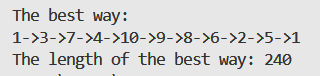
\includegraphics[]{комивояжер.png}
\centering
\caption{Результат работы программы}
\end{figure}